\chapter{Wavelets}
\label{app:wavelet}

\section{Introduction}
In the previous chapter, the \gls{fft} has been briefly described. It maps $N$ time-domain datapoints into $N$ frequency-domain datapoints. The \gls{fft} retain the information about the original signal, expressing it in the frequency domain. In other words, the \gls{fft} does not retain any knowledge about the time evolution of the signal and preserves the number of datapoints.

Another tool for signal processing is the wavelet. There are two main categories:
\begin{itemize}
\item  Wavelet Transform (\gls{wt}), which maps the datapoints of a 1D signal into a 2D plane, giving information about the frequency content of a signal at a given time.
\item Wavelet Packet Decomposition (\gls{wpd}), which is a tool that allows to decompose a signal into a tree of sub-bands, down-sampled signals. 
\end{itemize}

A mother wavelet is a function that complies with the following conditions:
\begin{align}
\int_{-\infty}^{\infty} \psi(t) dt = 0 & \qquad &\text{\gls{ie} it has a mean value of zero.} \\
\int_{-\infty}^{\infty} |\psi(t)|^2 dt = 1 & \qquad &\text{\gls{ie} it has a unitary energy.}
\end{align}

The Morlet wavelet is a complex wavelet, which complies with the above conditions. It is defined as:
\begin{equation}
\psi(t) = \frac{1}{\sqrt{\pi f_b}} e^{i 2 \pi f_c t} e^{-t^2/f_b} =  \frac{1}{\sqrt{\pi f_b}}[ \cos(2 \pi f_c t) + j\cdot \sin(2 \pi f_c t)] e^{-t^2/f_b}
\end{equation}
where $f_c$ is the central frequency and $f_b$ is the bandwidth. The Morlet wavelet is a complex wavelet, which means that it has a real and an imaginary part, as shown in Figure \ref{fig:morlet}. 

\begin{figure}
\centering
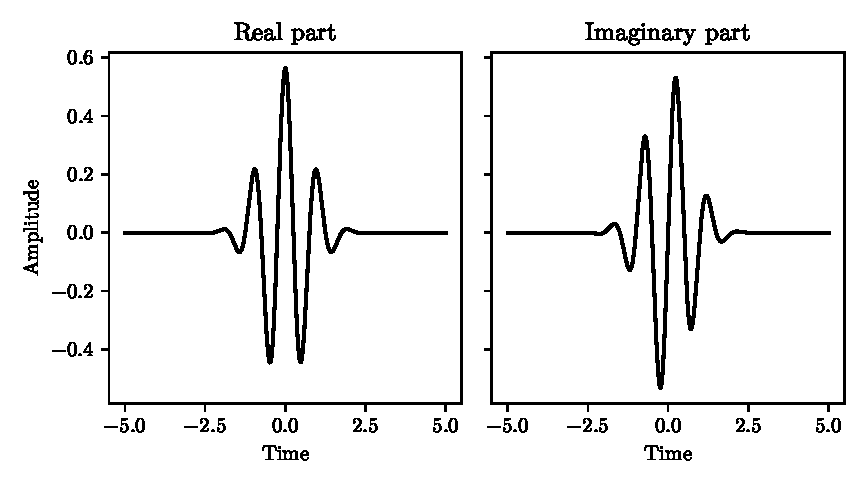
\includegraphics[]{images/morlet.pdf}
\caption{Real and imaginary part of the Morlet wavelet}
\label{fig:morlet}
\end{figure}
